% Generated by paper/build.mjs from public/data/results.json (2026-11-24T15:25:46.820Z). Do not edit.

\newcommand{\NRuns}{282}
\newcommand{\NLangs}{17}
\newcommand{\TotalCost}{74.72}
\newcommand{\NFailedRoundThree}{3}
\newcommand{\NFixed}{3}
\newcommand{\CostC}{1.31}
\newcommand{\OutC}{33\,266}
\newcommand{\CodeC}{22\,502}
\newcommand{\FirstC}{100}
\newcommand{\StdC}{0}
\newcommand{\ErrC}{0}
\newcommand{\MinC}{6.1}
\newcommand{\KvDiskC}{0.0}
\newcommand{\KvBuildC}{0.1}
\newcommand{\StdBuildC}{0.1}
\newcommand{\KvProjC}{0.0}
\newcommand{\KvWtC}{0.1}
\newcommand{\StdDiskC}{0.0}
\newcommand{\SpeedC}{1.32}
\newcommand{\CostCpp}{0.97}
\newcommand{\OutCpp}{21\,789}
\newcommand{\CodeCpp}{13\,469}
\newcommand{\FirstCpp}{100}
\newcommand{\StdCpp}{0}
\newcommand{\ErrCpp}{0}
\newcommand{\MinCpp}{5.9}
\newcommand{\KvDiskCpp}{0.8}
\newcommand{\KvBuildCpp}{1.1}
\newcommand{\StdBuildCpp}{0.4}
\newcommand{\KvProjCpp}{0.8}
\newcommand{\KvWtCpp}{3.2}
\newcommand{\StdDiskCpp}{0.0}
\newcommand{\SpeedCpp}{4.31}
\newcommand{\CostRust}{0.83}
\newcommand{\OutRust}{17\,277}
\newcommand{\CodeRust}{11\,721}
\newcommand{\FirstRust}{100}
\newcommand{\StdRust}{2}
\newcommand{\ErrRust}{0}
\newcommand{\MinRust}{5.1}
\newcommand{\KvDiskRust}{107}
\newcommand{\KvBuildRust}{11.4}
\newcommand{\StdBuildRust}{1.8}
\newcommand{\KvProjRust}{76}
\newcommand{\KvWtRust}{334}
\newcommand{\StdDiskRust}{1.3}
\newcommand{\SpeedRust}{2.44}
\newcommand{\CostGo}{0.85}
\newcommand{\OutGo}{18\,221}
\newcommand{\CodeGo}{12\,141}
\newcommand{\FirstGo}{100}
\newcommand{\StdGo}{0}
\newcommand{\ErrGo}{0}
\newcommand{\MinGo}{3.1}
\newcommand{\KvDiskGo}{115}
\newcommand{\KvBuildGo}{3.1}
\newcommand{\StdBuildGo}{1.5}
\newcommand{\KvProjGo}{5.6}
\newcommand{\KvWtGo}{132}
\newcommand{\StdDiskGo}{44}
\newcommand{\SpeedGo}{1.60}
\newcommand{\CostNim}{0.85}
\newcommand{\OutNim}{15\,954}
\newcommand{\CodeNim}{7\,378}
\newcommand{\FirstNim}{75}
\newcommand{\StdNim}{2}
\newcommand{\ErrNim}{0}
\newcommand{\MinNim}{5.6}
\newcommand{\KvDiskNim}{2.7}
\newcommand{\KvBuildNim}{1.2}
\newcommand{\StdBuildNim}{0.5}
\newcommand{\KvProjNim}{2.7}
\newcommand{\KvWtNim}{11}
\newcommand{\StdDiskNim}{0.6}
\newcommand{\SpeedNim}{2.79}
\newcommand{\CostZig}{1.96}
\newcommand{\OutZig}{39\,457}
\newcommand{\CodeZig}{16\,568}
\newcommand{\FirstZig}{100}
\newcommand{\StdZig}{21}
\newcommand{\ErrZig}{3}
\newcommand{\MinZig}{9.7}
\newcommand{\KvDiskZig}{67}
\newcommand{\KvBuildZig}{9.4}
\newcommand{\StdBuildZig}{5.4}
\newcommand{\KvProjZig}{22}
\newcommand{\KvWtZig}{133}
\newcommand{\StdDiskZig}{49}
\newcommand{\SpeedZig}{1.25}
\newcommand{\CostSwift}{1.58}
\newcommand{\OutSwift}{36\,578}
\newcommand{\CodeSwift}{15\,070}
\newcommand{\FirstSwift}{8}
\newcommand{\StdSwift}{4}
\newcommand{\ErrSwift}{6}
\newcommand{\MinSwift}{11.3}
\newcommand{\KvDiskSwift}{0.1}
\newcommand{\KvBuildSwift}{9.9}
\newcommand{\StdBuildSwift}{13.8}
\newcommand{\KvProjSwift}{0.1}
\newcommand{\KvWtSwift}{0.5}
\newcommand{\StdDiskSwift}{0.1}
\newcommand{\SpeedSwift}{4.11}
\newcommand{\CostJava}{0.88}
\newcommand{\OutJava}{18\,242}
\newcommand{\CodeJava}{10\,378}
\newcommand{\FirstJava}{83}
\newcommand{\StdJava}{0}
\newcommand{\ErrJava}{0}
\newcommand{\MinJava}{5.6}
\newcommand{\KvDiskJava}{0.0}
\newcommand{\KvBuildJava}{0.4}
\newcommand{\StdBuildJava}{0.3}
\newcommand{\KvProjJava}{0.0}
\newcommand{\KvWtJava}{0.1}
\newcommand{\StdDiskJava}{0.0}
\newcommand{\SpeedJava}{3.54}
\newcommand{\CostKotlin}{0.75}
\newcommand{\OutKotlin}{14\,080}
\newcommand{\CodeKotlin}{6\,795}
\newcommand{\FirstKotlin}{100}
\newcommand{\StdKotlin}{0}
\newcommand{\ErrKotlin}{0}
\newcommand{\MinKotlin}{5.6}
\newcommand{\KvDiskKotlin}{5.8}
\newcommand{\KvBuildKotlin}{4.3}
\newcommand{\StdBuildKotlin}{2.5}
\newcommand{\KvProjKotlin}{5.8}
\newcommand{\KvWtKotlin}{23}
\newcommand{\StdDiskKotlin}{5.8}
\newcommand{\SpeedKotlin}{3.99}
\newcommand{\CostCsharp}{1.28}
\newcommand{\OutCsharp}{28\,325}
\newcommand{\CodeCsharp}{12\,075}
\newcommand{\FirstCsharp}{8}
\newcommand{\StdCsharp}{1}
\newcommand{\ErrCsharp}{2}
\newcommand{\MinCsharp}{7.7}
\newcommand{\KvDiskCsharp}{277}
\newcommand{\KvBuildCsharp}{9.5}
\newcommand{\StdBuildCsharp}{13.1}
\newcommand{\KvProjCsharp}{223}
\newcommand{\KvWtCsharp}{937}
\newcommand{\StdDiskCsharp}{195}
\newcommand{\SpeedCsharp}{3.72}
\newcommand{\CostOdin}{1.21}
\newcommand{\OutOdin}{24\,656}
\newcommand{\CodeOdin}{11\,040}
\newcommand{\FirstOdin}{50}
\newcommand{\StdOdin}{0}
\newcommand{\ErrOdin}{2}
\newcommand{\MinOdin}{6.0}
\newcommand{\KvDiskOdin}{0.3}
\newcommand{\KvBuildOdin}{1.7}
\newcommand{\StdBuildOdin}{0.5}
\newcommand{\KvProjOdin}{0.3}
\newcommand{\KvWtOdin}{1.3}
\newcommand{\StdDiskOdin}{0.1}
\newcommand{\SpeedOdin}{1.39}
\newcommand{\CostOcaml}{0.91}
\newcommand{\OutOcaml}{19\,637}
\newcommand{\CodeOcaml}{10\,227}
\newcommand{\FirstOcaml}{92}
\newcommand{\StdOcaml}{1}
\newcommand{\ErrOcaml}{0}
\newcommand{\MinOcaml}{3.9}
\newcommand{\KvDiskOcaml}{3.5}
\newcommand{\KvBuildOcaml}{0.3}
\newcommand{\StdBuildOcaml}{0.2}
\newcommand{\KvProjOcaml}{3.5}
\newcommand{\KvWtOcaml}{14}
\newcommand{\StdDiskOcaml}{1.4}
\newcommand{\SpeedOcaml}{3.06}
\newcommand{\CostHaskell}{1.10}
\newcommand{\OutHaskell}{23\,785}
\newcommand{\CodeHaskell}{9\,758}
\newcommand{\FirstHaskell}{75}
\newcommand{\StdHaskell}{2}
\newcommand{\ErrHaskell}{1}
\newcommand{\MinHaskell}{7.2}
\newcommand{\KvDiskHaskell}{1467}
\newcommand{\KvBuildHaskell}{145.6}
\newcommand{\StdBuildHaskell}{0.4}
\newcommand{\KvProjHaskell}{103}
\newcommand{\KvWtHaskell}{1775}
\newcommand{\StdDiskHaskell}{20}
\newcommand{\SpeedHaskell}{4.51}
\newcommand{\CostJs}{0.73}
\newcommand{\OutJs}{14\,259}
\newcommand{\CodeJs}{6\,522}
\newcommand{\FirstJs}{100}
\newcommand{\StdJs}{0}
\newcommand{\ErrJs}{0}
\newcommand{\MinJs}{2.9}
\newcommand{\KvDiskJs}{0.0}
\newcommand{\KvBuildJs}{0.0}
\newcommand{\StdBuildJs}{0.0}
\newcommand{\KvProjJs}{0.0}
\newcommand{\KvWtJs}{0.0}
\newcommand{\StdDiskJs}{0.0}
\newcommand{\SpeedJs}{5.65}
\newcommand{\CostTs}{0.72}
\newcommand{\OutTs}{14\,127}
\newcommand{\CodeTs}{8\,437}
\newcommand{\FirstTs}{100}
\newcommand{\StdTs}{0}
\newcommand{\ErrTs}{0}
\newcommand{\MinTs}{2.7}
\newcommand{\KvDiskTs}{0.0}
\newcommand{\KvBuildTs}{0.0}
\newcommand{\StdBuildTs}{0.0}
\newcommand{\KvProjTs}{0.0}
\newcommand{\KvWtTs}{0.0}
\newcommand{\StdDiskTs}{0.0}
\newcommand{\SpeedTs}{6.14}
\newcommand{\CostPython}{0.69}
\newcommand{\OutPython}{12\,719}
\newcommand{\CodePython}{6\,632}
\newcommand{\FirstPython}{92}
\newcommand{\StdPython}{0}
\newcommand{\ErrPython}{0}
\newcommand{\MinPython}{2.8}
\newcommand{\KvDiskPython}{0.0}
\newcommand{\KvBuildPython}{0.0}
\newcommand{\StdBuildPython}{0.0}
\newcommand{\KvProjPython}{0.0}
\newcommand{\KvWtPython}{0.1}
\newcommand{\StdDiskPython}{0.0}
\newcommand{\SpeedPython}{6.52}
\newcommand{\CostAsm}{3.28}
\newcommand{\OutAsm}{99\,286}
\newcommand{\CodeAsm}{36\,769}
\newcommand{\FirstAsm}{58}
\newcommand{\StdAsm}{0}
\newcommand{\ErrAsm}{1}
\newcommand{\MinAsm}{15.8}
\newcommand{\KvDiskAsm}{0.0}
\newcommand{\KvBuildAsm}{0.1}
\newcommand{\StdBuildAsm}{0.1}
\newcommand{\KvProjAsm}{0.0}
\newcommand{\KvWtAsm}{0.1}
\newcommand{\StdDiskAsm}{0.0}
\newcommand{\SpeedAsm}{1.06}
\newcommand{\CorrCodeCost}{0.92}
\newcommand{\CorrCodeCostSpearman}{0.85}
\newcommand{\CorrCostSpeed}{0.63}
\newcommand{\FastestLang}{Assembly}
\newcommand{\KvPointsMin}{53}
\newcommand{\CorrCodeCostNoAsm}{0.71}
\newcommand{\TsJsCode}{1.29}
\newcommand{\TsJsCodeClk}{1.26}
\newcommand{\TsJsCost}{0.98}
\newcommand{\NTrackRuns}{60}
\newcommand{\NTrackLangs}{10}
\newcommand{\NTrackFailed}{0}
\newcommand{\NTrackFixed}{0}
\newcommand{\TrkNumericOctave}{0.48}
\newcommand{\TrkNumericJulia}{0.46}
\newcommand{\TrkNumericR}{0.31}
\newcommand{\TrkProofsLean}{0.28}
\newcommand{\TrkProofsRocq}{0.28}
\newcommand{\TrkProofsDafny}{0.25}
\newcommand{\TrkEvmSolidity}{0.42}
\newcommand{\TrkEvmVyper}{0.41}
\newcommand{\TrkZkCircom}{0.46}
\newcommand{\TrkZkNoir}{0.47}
\newcommand{\NSkillLangs}{0}
\newcommand{\NSkillCheaper}{0}
\newcommand{\NSkillWorksUp}{0}
\newcommand{\NSkillWorksDown}{0}
\newcommand{\SkillMedianChange}{--}
\newcommand{\SkillAuthorCost}{0.00}
\newcommand{\CorrStdCost}{0.32}
\newcommand{\DevloopRust}{206}
\newcommand{\DevloopRustWt}{857}
\newcommand{\NDepsLangs}{2}
\newcommand{\CheapestLang}{Python}
\newcommand{\CostCheapest}{0.69}
\newcommand{\ShortestLang}{JavaScript}
\newcommand{\RatioC}{1.9}
\newcommand{\RatioCpp}{1.4}
\newcommand{\RatioRust}{1.2}
\newcommand{\RatioGo}{1.2}
\newcommand{\RatioNim}{1.2}
\newcommand{\RatioZig}{2.9}
\newcommand{\RatioSwift}{2.3}
\newcommand{\RatioJava}{1.3}
\newcommand{\RatioKotlin}{1.1}
\newcommand{\RatioCsharp}{1.9}
\newcommand{\RatioOdin}{1.8}
\newcommand{\RatioOcaml}{1.3}
\newcommand{\RatioHaskell}{1.6}
\newcommand{\RatioJs}{1.1}
\newcommand{\RatioTs}{1.1}
\newcommand{\RatioPython}{1.0}
\newcommand{\RatioAsm}{4.8}
\newcommand{\ComboJsSvelte}{2\,736}
\newcommand{\ComboKotlinSvelte}{2\,775}
\newcommand{\ComboJsVue}{2\,790}
\newcommand{\ComboKotlinVue}{2\,829}
\newcommand{\ComboJsReact}{2\,994}
\newcommand{\ComboKotlinReact}{3\,033}
\newcommand{\ComboTsSvelte}{3\,219}
\newcommand{\ComboTsVue}{3\,273}
\newcommand{\ComboHaskellSvelte}{3\,308}
\newcommand{\ComboHaskellVue}{3\,362}
\newcommand{\ComboJavaSvelte}{3\,460}
\newcommand{\ComboTsReact}{3\,477}
\newcommand{\ComboJavaVue}{3\,514}
\newcommand{\ComboHaskellReact}{3\,566}
\newcommand{\ComboRustSvelte}{3\,702}
\newcommand{\ComboJavaReact}{3\,718}
\newcommand{\ComboRustVue}{3\,756}
\newcommand{\ComboRustReact}{3\,960}
\newcommand{\ComboNimSvelte}{4\,056}
\newcommand{\ComboNimVue}{4\,110}
\newcommand{\ComboPythonSvelte}{4\,148}
\newcommand{\ComboPythonVue}{4\,202}
\newcommand{\ComboNimReact}{4\,314}
\newcommand{\ComboPythonReact}{4\,406}
\newcommand{\ComboCsharpSvelte}{4\,432}
\newcommand{\ComboCsharpVue}{4\,486}
\newcommand{\ComboCsharpReact}{4\,690}
\newcommand{\ComboGoSvelte}{5\,442}
\newcommand{\ComboGoVue}{5\,496}
\newcommand{\ComboGoReact}{5\,700}
\newcommand{\ComboOdinSvelte}{5\,810}
\newcommand{\ComboOdinVue}{5\,864}
\newcommand{\ComboOcamlSvelte}{6\,006}
\newcommand{\ComboOcamlVue}{6\,060}
\newcommand{\ComboOdinReact}{6\,068}
\newcommand{\ComboOcamlReact}{6\,264}
\newcommand{\ComboSwiftSvelte}{8\,017}
\newcommand{\ComboSwiftVue}{8\,071}
\newcommand{\ComboSwiftReact}{8\,275}
\newcommand{\ComboZigSvelte}{8\,565}
\newcommand{\ComboZigVue}{8\,619}
\newcommand{\ComboCppSvelte}{8\,637}
\newcommand{\ComboCppVue}{8\,691}
\newcommand{\ComboZigReact}{8\,823}
\newcommand{\ComboCppReact}{8\,895}
\newcommand{\ComboCSvelte}{12\,743}
\newcommand{\ComboCVue}{12\,797}
\newcommand{\ComboCReact}{13\,001}
\newcommand{\ComboAsmSvelte}{16\,803}
\newcommand{\ComboAsmVue}{16\,857}
\newcommand{\ComboAsmReact}{17\,061}

\newcommand{\LeaderboardTable}{%
\begin{tabular}{@{}lrrrrrrrrr@{}}
\toprule
Language & Solved & 1st try & US\$ & Output & Turns & Min & Code & Errors & Stdlib \\
\midrule
Python & 12/12 & 92\% & 0.69 & 12\,719 & 17 & 2.8 & 6\,632 & 0.0 & 0 \\
TypeScript & 12/12 & 100\% & 0.72 & 14\,127 & 16 & 2.7 & 8\,437 & 0.0 & 0 \\
JavaScript & 12/12 & 100\% & 0.73 & 14\,259 & 17 & 2.9 & 6\,522 & 0.0 & 0 \\
Kotlin & 12/12 & 100\% & 0.75 & 14\,080 & 20 & 5.6 & 6\,795 & 0.0 & 0 \\
Rust & 12/12 & 100\% & 0.83 & 17\,277 & 18 & 5.1 & 11\,721 & 0.0 & 2 \\
Nim & 12/12 & 75\% & 0.85 & 15\,954 & 23 & 5.6 & 7\,378 & 0.0 & 2 \\
Go & 12/12 & 100\% & 0.85 & 18\,221 & 17 & 3.1 & 12\,141 & 0.0 & 0 \\
Java & 12/12 & 83\% & 0.88 & 18\,242 & 22 & 5.6 & 10\,378 & 0.0 & 0 \\
OCaml & 12/12 & 92\% & 0.91 & 19\,637 & 25 & 3.9 & 10\,227 & 0.0 & 1 \\
C++ & 12/12 & 100\% & 0.97 & 21\,789 & 20 & 5.9 & 13\,469 & 0.0 & 0 \\
Haskell & 12/12 & 75\% & 1.10 & 23\,785 & 33 & 7.2 & 9\,758 & 1.0 & 2 \\
Odin & 9/12 & 50\% & 1.21 & 24\,656 & 37 & 6.0 & 11\,040 & 2.0 & 0 \\
C\# & 12/12 & 8\% & 1.28 & 28\,325 & 36 & 7.7 & 12\,075 & 2.0 & 1 \\
C & 12/12 & 100\% & 1.31 & 33\,266 & 25 & 6.1 & 22\,502 & 0.0 & 0 \\
Swift & 12/12 & 8\% & 1.58 & 36\,578 & 39 & 11.3 & 15\,070 & 6.0 & 4 \\
Zig & 12/12 & 100\% & 1.96 & 39\,457 & 48 & 9.7 & 16\,568 & 3.0 & 21 \\
Assembly & 12/12 & 58\% & 3.28 & 99\,286 & 37 & 15.8 & 36\,769 & 1.0 & 0 \\
\bottomrule
\end{tabular}}

\newcommand{\CostPlot}{%
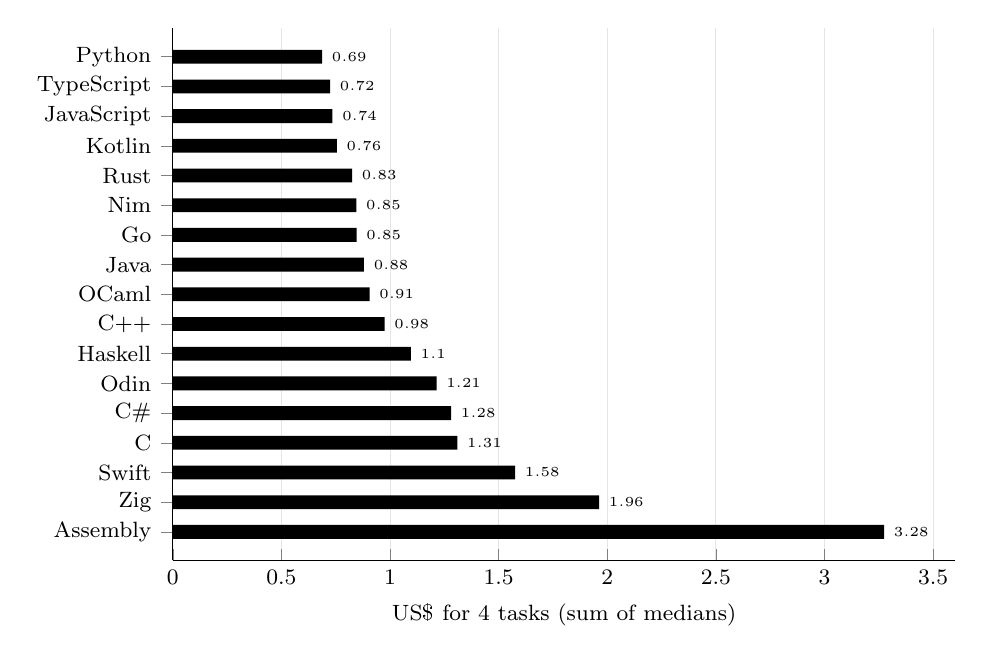
\begin{tikzpicture}
\begin{axis}[xbar, width=0.95\columnwidth, height=8.34cm, bar width=5pt, xmin=0,
  symbolic y coords={Asm,Zig,Swift,C,Csharp,Odin,Haskell,Cpp,Ocaml,Java,Go,Nim,Rust,Kotlin,Js,Ts,Python}, ytick=data, yticklabels={Assembly,Zig,Swift,C,C\#,Odin,Haskell,C++,OCaml,Java,Go,Nim,Rust,Kotlin,JavaScript,TypeScript,Python},
  xlabel={US\$ for 4 tasks (sum of medians)}, nodes near coords, nodes near coords style={font=\tiny}, every node near coord/.append style={/pgf/number format/.cd, fixed, precision=2, use period},
  tick label style={font=\footnotesize}, label style={font=\footnotesize}, axis x line*=bottom, axis y line*=left, enlarge y limits=0.06, xmajorgrids, major grid style={gray!20}]
\addplot[fill=black, draw=none] coordinates {(3.275,Asm) (1.963,Zig) (1.576,Swift) (1.310,C) (1.281,Csharp) (1.214,Odin) (1.096,Haskell) (0.975,Cpp) (0.906,Ocaml) (0.880,Java) (0.846,Go) (0.845,Nim) (0.825,Rust) (0.755,Kotlin) (0.735,Js) (0.724,Ts) (0.687,Python)};
\end{axis}
\end{tikzpicture}}

\newcommand{\CodePlot}{%
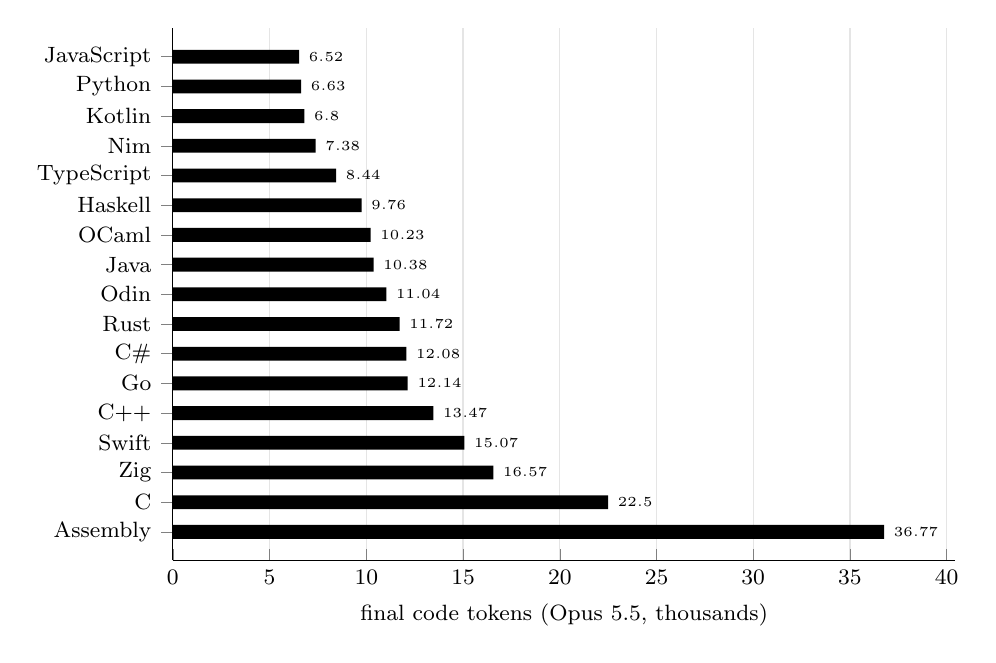
\begin{tikzpicture}
\begin{axis}[xbar, width=0.95\columnwidth, height=8.34cm, bar width=5pt, xmin=0,
  symbolic y coords={Asm,C,Zig,Swift,Cpp,Go,Csharp,Rust,Odin,Java,Ocaml,Haskell,Ts,Nim,Kotlin,Python,Js}, ytick=data, yticklabels={Assembly,C,Zig,Swift,C++,Go,C\#,Rust,Odin,Java,OCaml,Haskell,TypeScript,Nim,Kotlin,Python,JavaScript},
  xlabel={final code tokens (Opus 5.5, thousands)}, nodes near coords, nodes near coords style={font=\tiny}, every node near coord/.append style={/pgf/number format/.cd, fixed, precision=2, use period},
  tick label style={font=\footnotesize}, label style={font=\footnotesize}, axis x line*=bottom, axis y line*=left, enlarge y limits=0.06, xmajorgrids, major grid style={gray!20}]
\addplot[fill=black, draw=none] coordinates {(36.769,Asm) (22.502,C) (16.568,Zig) (15.070,Swift) (13.469,Cpp) (12.141,Go) (12.075,Csharp) (11.721,Rust) (11.040,Odin) (10.378,Java) (10.227,Ocaml) (9.758,Haskell) (8.437,Ts) (7.378,Nim) (6.795,Kotlin) (6.632,Python) (6.522,Js)};
\end{axis}
\end{tikzpicture}}

\newcommand{\KvTable}{%
\begin{tabular}{@{}l>{\raggedright\arraybackslash}p{3.6cm}rrr@{}}
\toprule
Language & Dependencies (most common) & MB & Build s & req/s \\
\midrule
Haskell & bytestring, containers, http-types, wai, warp & 1467 & 145.6 & 23\,610 \\
C\# & stdlib & 277 & 9.5 & 22\,434 \\
Go & stdlib & 115 & 3.1 & 24\,521 \\
Rust & bytes, http-body-util, hyper, hyper-util, tokio & 107 & 11.4 & 17\,513 \\
Zig & stdlib & 67 & 9.4 & 26\,144 \\
Kotlin & stdlib & 5.8 & 4.3 & 21\,422 \\
OCaml & stdlib & 3.5 & 0.3 & 24\,709 \\
Nim & stdlib & 2.7 & 1.2 & 22\,069 \\
C++ & stdlib & 0.8 & 1.1 & 24\,017 \\
Odin & stdlib & 0.3 & 1.7 & 23\,677 \\
Swift & stdlib & 0.1 & 9.9 & 14\,837 \\
C & stdlib & 0.0 & 0.1 & 27\,776 \\
Java & stdlib & 0.0 & 0.4 & 22\,763 \\
Assembly & stdlib & 0.0 & 0.1 & 22\,051 \\
Python & stdlib & 0.0 & 0.0 & 27\,272 \\
JavaScript & stdlib & 0.0 & 0.0 & 24\,608 \\
TypeScript & stdlib & 0.0 & 0.0 & 25\,275 \\
\bottomrule
\end{tabular}}

\newcommand{\PerfTable}{%
\begin{tabular}{@{}lrrrr@{}}
\toprule
Language & wordfreq ms & lru ms & calc ms & lru RSS MB \\
\midrule
Assembly & 94 & 36 & 18 & 29 \\
Zig & 119 & 56 & 21 & 28 \\
Odin & 158 & 59 & 21 & 39 \\
C & 135 & 52 & 26 & 30 \\
Go & 169 & 80 & 26 & 20 \\
Rust & 244 & 180 & 31 & 42 \\
Nim & 308 & 245 & 39 & 58 \\
OCaml & 366 & 241 & 54 & 18 \\
Haskell & 1\,100 & 218 & 89 & 117 \\
Swift & 194 & 525 & 91 & 8.5 \\
C\# & 315 & 330 & 91 & 113 \\
Java & 182 & 290 & 149 & 138 \\
Kotlin & 230 & 349 & 149 & 152 \\
JavaScript & 837 & 350 & 188 & 262 \\
TypeScript & 861 & 365 & 251 & 285 \\
C++ & 200 & 223 & 406 & 43 \\
Python & 607 & 346 & 516 & 184 \\
\bottomrule
\end{tabular}}

\newcommand{\SpeedTable}{%
\begin{tabular}{@{}rlrrrrrr@{}}
\toprule
\# & Language & wordfreq & lru & calc & kvhttp & Score & $\times$fastest \\
\midrule
1 & Assembly & 100 & 100 & 100 & 79 & \textbf{94.4} & 1.06 \\
2 & Zig & 79 & 64 & 86 & 94 & \textbf{80.0} & 1.25 \\
3 & C & 70 & 69 & 69 & 100 & \textbf{76.0} & 1.32 \\
4 & Odin & 59 & 61 & 86 & 85 & \textbf{71.8} & 1.39 \\
5 & Go & 56 & 45 & 69 & 88 & \textbf{62.5} & 1.60 \\
6 & Rust & 39 & 20 & 58 & 63 & \textbf{41.0} & 2.44 \\
7 & Nim & 31 & 15 & 46 & 79 & \textbf{35.8} & 2.79 \\
8 & OCaml & 26 & 15 & 33 & 89 & \textbf{32.7} & 3.06 \\
9 & Java & 52 & 12 & 12 & 82 & \textbf{28.2} & 3.54 \\
10 & C\# & 30 & 11 & 20 & 81 & \textbf{26.9} & 3.72 \\
11 & Kotlin & 41 & 10 & 12 & 77 & \textbf{25.0} & 3.99 \\
12 & Swift & 48 & 7 & 20 & 53 & \textbf{24.3} & 4.11 \\
13 & C++ & 47 & 16 & 4 & 86 & \textbf{23.2} & 4.31 \\
14 & Haskell & 9 & 17 & 20 & 85 & \textbf{22.2} & 4.51 \\
15 & JavaScript & 11 & 10 & 10 & 89 & \textbf{17.7} & 5.65 \\
16 & TypeScript & 11 & 10 & 7 & 91 & \textbf{16.3} & 6.14 \\
17 & Python & 15 & 10 & 3 & 98 & \textbf{15.3} & 6.52 \\
\bottomrule
\end{tabular}}

\newcommand{\FrontTable}{%
\begin{tabular}{@{}lrrrrr>{\raggedright\arraybackslash}p{3cm}@{}}
\toprule
 & Article & Ours & Ours & ui & shop & Store in shop \\
 & cl100k & cl100k & Opus & tokens & tokens & (agent's choice) \\
\midrule
React & 1.254 & 1.217 & 1.264 & 2\,599 & 3\,348 & Context + useReducer \\
Svelte & 1.000 & 1.000 & 1.000 & 2\,056 & 2\,543 & Svelte runes (\$state) \\
Vue & 1.115 & 1.090 & 1.108 & 2\,278 & 2\,581 & Vue reactive(), Pinia \\
\bottomrule
\end{tabular}}

\newcommand{\TrackTable}{%
\begin{tabular}{@{}llrrrrrrr@{}}
\toprule
Track & Language & Solved & Repaired & 1st try & US\$ & Output & Code & Turns \\
\midrule
Scientific computing & R & 6/6 & 6/6 & 100\% & 0.31 & 4\,329 & 2\,135 & 10 \\
 & Julia & 6/6 & 6/6 & 83\% & 0.46 & 9\,867 & 5\,386 & 10 \\
 & Octave & 6/6 & 6/6 & 100\% & 0.48 & 8\,596 & 1\,923 & 20 \\
\midrule
Theorem proving & Dafny & 6/6 & 6/6 & 100\% & 0.25 & 2\,285 & 2\,260 & 7 \\
 & Lean 4 & 6/6 & 6/6 & 83\% & 0.28 & 2\,777 & 1\,892 & 9 \\
 & Rocq & 6/6 & 6/6 & 100\% & 0.28 & 2\,944 & 2\,043 & 8 \\
\midrule
Smart contracts & Vyper & 6/6 & 6/6 & 100\% & 0.41 & 5\,757 & 3\,973 & 9 \\
 & Solidity & 6/6 & 6/6 & 100\% & 0.42 & 5\,947 & 3\,432 & 8 \\
\midrule
Zero-knowledge circuits & Circom & 6/6 & 6/6 & 83\% & 0.46 & 8\,613 & 3\,032 & 13 \\
 & Noir & 6/6 & 6/6 & 33\% & 0.47 & 7\,330 & 3\,169 & 12 \\
\bottomrule
\end{tabular}}

\newcommand{\SkillTable}{%
\begin{tabular}{@{}lrrrrrrrr@{}}
\toprule
Language & Works & US\$ & $\Delta$US\$ & $\Delta$Output & Errors & Used & Skill US\$ & Pays off \\
\midrule

\bottomrule
\end{tabular}}

\newcommand{\SkillSlope}{%
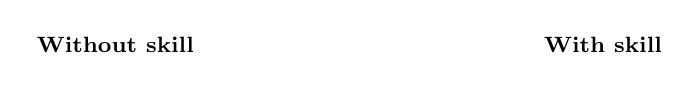
\begin{tikzpicture}
\node[anchor=east, font=\footnotesize\bfseries] at (-0.1,0.5) {Without skill};
\node[anchor=west, font=\footnotesize\bfseries] at (4.1,0.5) {With skill};

\end{tikzpicture}}
